
\documentclass[a4paper]{report}
% \documentclass{report}
\usepackage[utf8]{inputenc}
\usepackage{amsmath}
\usepackage{esint}
\usepackage{tabstackengine}
\usepackage[colorlinks,linkcolor=blue]{hyperref}
\usepackage{xeCJK}
\usepackage{caption}
\usepackage{stackengine}
\usepackage{graphicx}
\graphicspath{ {../resources/figure/dsp/} }
\usepackage{float}
\usepackage{amsmath}
\usepackage{ulem}
\usepackage{amsfonts}
\usepackage{blkarray}
\usepackage{enumitem}
\setlist[1]{itemsep=-5pt}
\usepackage{subcaption}

\usepackage{tikz}
\usetikzlibrary{calc}
\usepackage{pgfplots}
\usepackage{mathrsfs}
\usepackage{multirow}
\usetikzlibrary{shapes,arrows,positioning}
\captionsetup[table]{skip=10pt}

%%%% 下面的命令重定义页面边距,使其符合中文刊物习惯 %%%%
\addtolength{\topmargin}{-54pt}
\setlength{\oddsidemargin}{0.63cm}  % 3.17cm - 1 inch
\setlength{\evensidemargin}{\oddsidemargin}
\setlength{\textwidth}{14.66cm}
\setlength{\textheight}{24.00cm}    % 24.62


% 段首不缩进
\setlength{\parindent}{0pt}
%%%% 下面的命令设置行间距与段落间距 %%%%
\linespread{1.2}
% \setlength{\parskip}{1ex}
\setlength{\parskip}{.5\baselineskip}

\def\rlwd{.5pt} \def\rlht{2.2ex} \def\rldp{.5ex}
\def\mydiv#1{~%
  \rule[-\rldp]{\rlwd}{\rlht}%
  \setbox0=\hbox{~#1}%
  \stackunder[\dimexpr\rldp-\rlwd]{~#1}{\rule{\wd0}{\rlwd}}%
}

\title{DSP}
\author{Crosstyan}
\date{Dec 2020}


\begin{document}
\chapter{Discrete Time Domain}
\section{常用序列}
既然是离散的, 我们就默认$n\in \textbf{Z}$
\subsection{Unit Impulse Sequence}
\begin{equation}
    \delta(n)=
  \begin{cases}
    0 & n=0
    \\ 1 & n\neq 1
  \end{cases}
\end{equation}
\subsection{Unit Step Sequence}
\begin{equation}
  u(n)=\begin{cases}
    1& n\geq 0
    \\ 0& n<0
  \end{cases}
\end{equation}
\subsection{Rectangle Sequence}
\begin{equation}
  R_N(n)=\begin{cases}
    1 & 0\leq n\leq N-1
    \\ 0 & \text{elsewhere}
  \end{cases}
\end{equation}
说人话就是在$[0,N-1]$上面都是1. 
\subsection{Periodic Sequence}
存在正整数, 使得
\begin{equation}
  x(n)=x(n+N)
\end{equation}
成立.

怎么判断一个序列是否为Sinusoidal的以及找一个Sinusoidal序列的最小正周期呢? 

周期$\omega$里面带有$\pi$的基本都是周期函数. 
$$\omega\cdot N=2\pi k\quad\quad k\in \textbf{Z}$$
找到一个$k$使得的最小正整数$N$满足$N=\frac{2\pi k}{\omega}$ ($k\in \textbf{Z}$)

\section{Pearson correlation coefficient}
相关系数, 对长度为$N$的$[0,N-1]$的点进行采样. 
\begin{align*}
  r=\frac{\displaystyle\sum_{n=0}^{N-1}x(n)\cdot y^*(n)}{\sqrt{\displaystyle\sum_{n=0}^{N-1}\lvert x(n)\rvert^2\cdot  \displaystyle\sum_{n=0}^{N-1}\lvert y(n)\rvert^2}}
\end{align*}
$y^*(n)$为$y(n)$的共轭, 一般$x(n)$和$y(n)$都是实数啦\dots
\section{cross-correlation}
相关序列, 互相关. 
\subsection{相关序列与卷积关系}

\begin{align*}
  x(n)* h(n)&=\displaystyle\sum_{k=0}^{N-1} h(k)\cdot x(n-k)
  \\ \text{corr}[x(n),h(n)]&=\displaystyle\sum_{k=0}^{N-1} h(k)\cdot x(n+k)
\end{align*}
The only difference between cross-correlation and convolution is a time reversal on one of the inputs. 

互相关函数和卷积运算几乎一样,但没有对核进行翻转。Kernel如果是对称的,cross-correlation跟convolution恰好效果是一样的。

\section{System}
\begin{equation}
  y(n)=T[x(n)]
\end{equation}
\subsection{Properties}
\subsubsection{Linear}
\begin{equation}
  T[a\cdot x_1(n)+b\cdot x_2(n)]=a\cdot T[x_1(n)]+b\cdot T[x_1(n)]
\end{equation}
\subsubsection{Time Invariant}
变换后时移等于时移后变换
\begin{equation}
  y(n-k)=T[x](n-k)=T[x(n-k)]
\end{equation}
类似$y(n)=T[x(n)]=x(2\cdot n)$或者$y(n)=n\cdot x(n)$都是时变系统. 
\subsubsection{Causality}
Impulse Response equals zero when $t<0$. 
\begin{equation}
  T[\delta(n)]=h(n)
\end{equation}
\subsubsection{Stability}
输入有界输出亦有界
\subsection{Unit Impulse Response}
假设一个系统\footnote{看作是变换函数的函数, 或者说是泛函数; 或者是一个黑箱子, 丢进去某些参数, 送出来某些输出}(或者变换)\footnote{「$\cdot$」代表被变换的玩意, 或者系统的输入}为$T[\cdot]$, 把一个脉冲(Impulse) $\delta(n)$丢进去, 出来的玩意就被叫做单位脉冲响应. 所谓「响应」就是指系统给与某一特定输入的输出. 
\begin{equation}
  h(n)=T[\delta(n)]
\end{equation}
$h(n)$就代表了把$\delta(n)$丢到系统$T[\cdot]$之后的输出. $h(n)$就代表了一个系统, 只要说到$h(n)$, 就等同于指代那个系统$T[\cdot]$.
\subsection{Linear Convolution}
我们想知道$x(n)$经过Unit Impulse Response为$h(n)$的输出$y(n)$是什么. 
\begin{equation}
  y(n)=x(n) * h(n)
\end{equation}
「*」代表线性卷积
\begin{equation}
  x(n) * h(n)=\displaystyle\sum_{k=-\infty}^{\infty}x(k)\cdot h(n-k)
\end{equation}
假设序列$x(n)$的长度为$N$, $h(n)$的长度为$M$, 则线性卷积的结果的长度为$M+N-1$
\subsection{圆周卷积}
又被称作N点周期卷积, 或者循环卷积

假设序列$x(n)$的周期为$N$, $h(n)$的周期也为$N$, 若两者长度不一致则需要将短的补零来补齐, 圆周卷积的结果的长度也为$N$
\begin{equation}
  (x \otimes h)[n]=\displaystyle\sum_{k=0}^{N}x(k)\cdot h[(n-k)_N]
\end{equation}
其中$(n-k)_N$表示$n-k$对$N$取模
\subsubsection{Properties}
\begin{itemize}
  \item 交换律
  \item 结合律
  \item 分配律
  \item 标量乘 $a\cdot (f*g)=(a\cdot f)* g$
  \item 位移(Impulse Convolution) $f(n)*\delta(n-D)=f(n-D)$
\end{itemize}
\subsection{Differential Equation}
\begin{equation}
  y(n)=\displaystyle\sum_{j=0}^{J}b_j\cdot x(n-j)-\displaystyle\sum_{i=1}^{I} a_i\cdot y(n-i)
\end{equation}
若$I=0$, 则被称作$J$阶差分方程. 
\section{采样定理}
设$T_s$为采样周期, 那么采样频率$f_s$为
\begin{equation}
  f_s=\frac{1}{T_s}
\end{equation}
模拟角频率$\Omega$和数字角频率$\omega$的转换关系为
\begin{equation}
  \omega=\Omega\cdot T_s
\end{equation}
$f$ 一般代表模拟频率. 当采样频率等于信号最高频率$f_H$的两倍时, 采样频率为 Nyquist 频率
\begin{equation}
  f_s=f_{\text{Nyquist}}=2\cdot f_H
\end{equation}
当使用带通滤波器时, 若信号的最高频率为$f_H$, 最低频率为$f_L$, 有最小采样频率(奈奎斯特频率)$f_s$
\begin{equation}
  f_{s}=2\cdot (f_H-f_L)
\end{equation}
\section{不失真系统}
\begin{equation}
  H(\omega)=k\cdot e^{-j\cdot \omega\cdot m}
\end{equation}
即系统的频率响应: 幅度响应为常数, 相位响应为过零点的直线
\chapter{Frequency Domain and Z Transformation}
\section{Fourier Transform}
按照周期(非周期)和连续(离散), 信号可以分为几类

假设$n$为时序, $k$为频序, $\omega$为数字角频率, $\Omega$为模拟角频率

如果你的频域是离散的,那么就有一个最小的分辨频率,这个自然对应了时域的最大周期,即时域的周期性。
反之同理。如果你的时域是离散的,那就有一个最小的周期。这个周期就对应频域的最高频率。所有高于这个频率的信息,都要被alias、反褶到低频去。即频域的周期性。
\subsection{Aperiodic Continuous}
Fourier Transform. 傅里叶变换\footnote{会把FT或者DTFT的结果用$X(\omega)$或者$X(e^{j\omega})$表示. 两者大概差不多是同一个意思. $\omega$表示数字角频率(时域离散), $\Omega$表示模拟角频率(时域连续)}
\begin{equation}
  X(e^{j\Omega})=\int_{-\infty}^\infty x(t)\cdot e^{-j\Omega\cdot t}\; dt
\end{equation}
\subsection{Periodic Continuous}
Fourier Series. 傅里叶级数. 

假设最小正周期为$T$
\begin{equation}
  X(k)=\frac{1}{T}\cdot\int_0^T x(t)\cdot e^{-j\cdot\frac{2\pi}{T}\cdot k\cdot t} \; dt
\end{equation}

\subsection{Aperiodic Discrete}
Discrete Time Fourier Transform (DTFT), 离散时间傅里叶变换
\begin{equation}
  X(e^{j\omega})=\displaystyle\sum_{n=-\infty}^\infty x(n)\cdot e^{-j\omega\cdot n}\; 
\end{equation}
反变换
\begin{equation}
  x(n)=\frac{1}{2\pi}\int_0^{2\pi}X(\omega)\cdot e^{j\omega n} \;\text{d}\omega
\end{equation}
\subsection{Periodic Discrete}
Discrete Fourier Series (DFS) 离散傅里叶级数. 

假设最小正周期为$N$, 频序为$k$
\begin{equation}
  X(k)=\displaystyle\sum_{n=0}^{N-1}x(n)\cdot e^{-j\cdot\frac{2\pi}{N}\cdot k\cdot n}
\end{equation}

或者取DFS的主值区间得到 Discrete Fourier Transform (DFT). 离散傅里叶变换. 

% 其中正弦波的复数幅度为
% \begin{equation}
%   X(k)=\frac{1}{N}\displaystyle\sum_{n=0}^{N-1}x(n)\cdot e^{-j\cdot\frac{2\pi}{N}\cdot k\cdot n}
% \end{equation}
\section{DTFT}
既然是Digital Signal Processing. 那么就只讨论离散(Discrete)的情况, 一般的信号都是Aperiodic(非周期的). 所以让我们来讨论DTFT罢! 

% Table generated by Excel2LaTeX from sheet 'Sheet1'
\begin{table}[H]
  \centering
    \begin{tabular}{ccc}
    Time Domain & Frequency Domain & Transform \\
    \hline
    Aperiodic & Continuous & DTFT\\
    Periodic & Discrete & DFS \\
    \end{tabular}%
  \caption{非连周离}
\end{table}%

这样就建立起了时域与频域的关系, 时域非周期, 频域连续; 时域周期, 频域离散\footnote{离散才能写成级数(多项式)的形式啦\dots 也可以说DFS是一种特殊的DFT? }. 

下面给出DTFT的定义式
\begin{equation}
  X(e^{j\omega})=DTFT[x(n)]=\displaystyle\sum_{n=-\infty}^{\infty}x(n)\cdot e^{-j\omega\cdot n}
\end{equation}

\begin{table}[H]
  \centering
    \begin{tabular}{cc}
    Time Domain $x(n)$ & Frequency Domain $X(e^{j\omega})$ \\
    \hline
    $\delta(n)$ & 1 \\
    $\delta(n-k)$ & $e^{-j\omega\cdot k}$  \\
    $R_N(n)$&$\frac{\sin{\frac{N\cdot\omega}{2}}}{\sin{\frac{\omega}{2}}}\cdot e^{-j\cdot\frac{N-1}{2}\cdot\omega}$
    \end{tabular}%
  \caption{常用傅里叶变换对}
\end{table}%

\begin{table}[H]
  \centering
    \begin{tabular}{ccc}
    性质& $x(n)$ &  $X(e^{j\omega})$ \\
    \hline
    线性&$a\cdot x(n)\pm b\cdot y(n)$ & $a\cdot X(e^{j\omega})\pm b\cdot Y(e^{j\omega})$ \\
    时移&$x(n-m)$ & $e^{-j\omega\cdot m}\cdot X(e^{j\omega})$  \\
    时域卷积 & $x(n)*h(n)$ & $X(e^{j\omega})\cdot H(e^{j\omega})$\\
    频域卷积 & $x(n)\cdot h(n)$ & $\frac{1}{2\pi}X(e^{j\omega})* H(e^{j\omega})$\\
    频域微分 & $n\cdot x(n)$ & $j\cdot \frac{\text{d} X(e^{j\omega})}{\text{d}\omega}$
    \end{tabular}%
  \caption{常用傅里叶变换性质}
\end{table}%
\subsection{频谱的对称}
前提是输入的序列为\textbf{实数序列}\footnote{不过我们一般也只讨论实数序列}. 实数序列的对称性让$\omega$的主值区间从$[0,2\pi)$缩小到$[0,\pi]$, 让$k$的主值区间由$[0,N)$缩小到$[0,\frac{N}{2}]$, 减小了一半的工作量. 
\subsection{幅频特性偶对称}
\begin{equation}
  \lvert X(e^{j\omega})\rvert =\lvert X(e^{-j\omega})\rvert
\end{equation}
\subsection{相频特性奇对称}
\begin{equation}
  \arg [X(e^{j\omega})] =-\arg [X(e^{-j\omega})]
\end{equation}
% \subsection{频谱搬移}
% \begin{equation}
%   X(N-k)=X(-k)
% \end{equation}
\section{Z Transform}
序列的傅里叶变换是单位圆上的z变换
$$X(e^{j\omega})=X(z)\mid_{z=e^{j\omega}}$$
收敛域(收敛半径, Radius of Converge), 又称ROC. 

因果稳定系统, $H(z)$全部极点都在单位圆\footnote{半径为1的圆}, 且ROC在单位圆外的系统. (单位圆包含在ROC之内)

如果你要稳定性,收敛域必须包含单位圆;如果你需要一个因果系统,收敛域必须包含无穷大. 如果你既要稳定性,也要因果性,系统函数的所有极点都必须在单位圆内。

也就是ROC为
\begin{equation}
  \begin{cases}
    \lvert z \rvert > a \\
    a < 1
  \end{cases}
\end{equation}

啥叫零点极点? 一个系统可以写成这种形式\footnote{一般是输出比上输入啦\dots}
\begin{equation}
  H(z)=\frac{Y(z)}{X(z)}=K\cdot\frac{(z-z_1)\cdot(z-z_2)\dots (z-z_{m-1})\cdot (z-z_{m})}{(z-p_1)\cdot(z-p_2)\dots (z-p_{n-1})\cdot (z-p_{n})}
\end{equation}
\paragraph{零点} 使得$H(z)\rightarrow 0$的点, 也就是$z_1,\; z_2\dots z_m$, 系统分子多项式的根
\paragraph{极点} 使得$H(z)\rightarrow \infty$的点, 也就是$p_1,\; p_2\dots p_n$, 系统分母多项式的根

\begin{table}[H]
  \centering
    \begin{tabular}{ccc}
    $x(n)$ & $X(z)$&ROC \\
    \hline
    $\delta(n)$ & 1 & 所有值$z$\\
    $a^n\cdot u(n)$ & $\frac{1}{1-a\cdot z^{-1}}$&$\lvert z\rvert >\lvert a\rvert$  \\
    $\sin(\theta)\cdot u(n)$&$\frac{\sin(\theta)\cdot z^{-1}}{1-2\cos(\theta)\cdot z^{-1}\cdot +z^{-2}}$&$\lvert z\rvert >1$
    \\     $\cos(\theta)\cdot u(n)$&$\frac{1-\cos(\theta)\cdot z^{-1}}{1-2\cos(\theta)\cdot z^{-1}\cdot +z^{-2}}$&$\lvert z\rvert >1$
    \end{tabular}%

  \caption{常用z变换对}
\end{table}%

\subsection{差分方程和Z变换}
首先要知道延时和z变换的关系
\begin{equation}
  a\cdot y(n-k)=Y(z)\cdot(a\cdot z^{-k})
\end{equation}
把差分方程进行z变换之后把$X(z)$和$Y(z)$提出来然后变换成为$\frac{Y(z)}{X(z)}$即可. 
\subsection{零极点图}
画个单位圆, 零点打圈$\circ$, 极点打叉$\times$. 零点阻碍对应的频率成分通过系统, 极点帮助对应的频率成分通过系统. 也就是说零点所在频率被抑制, 极点所在频率成分被提升. 

\subsubsection{幅频特性曲线}
假设有$m$个零点, $n$个极点
\begin{equation}
  \lvert H(\omega)\rvert=\lvert H(z)\rvert_{z=e^{j\omega}}=K\cdot \frac{\displaystyle\prod_{i=1}^{m}\lvert z-z_i\rvert}{\displaystyle\prod_{i=1}^{n}\lvert z-p_i\rvert}
\end{equation}
代表对应$\omega$频率下的幅频特性. 一般只取下面三个典型的$\omega$进行计算. 
\begin{itemize}
  \item $\omega=0$ 代表低频
  \item $\omega=\frac{\pi}{2}$ 代表中频
  \item $\omega=\pi$ 代表高频
\end{itemize}
\paragraph{零点矢量和极点矢量}零点矢量就是零点到$e^{j\omega}$的连线, 极点矢量同理. 
而我们得画$e^{j\cdot 0}$, $e^{j\cdot \frac{\pi}{2}}$, $e^{j\cdot \pi}$三个零极点图\footnote{$e^{j0}=1, e^{j\frac{\pi}{2}=j, e^{j\pi}=-1}$}, 找出其零点矢量和极点矢量的长度, 也就得到了$\lvert z-z_i\rvert$和$\lvert z-p_i\rvert$, 带入增益公式即可. 

若题目给出系统的幅频特性最大值\footnote{一般都是1啦\dots}为$G_{\max}$, 那就先算被提升的那一频段$\lvert H(\omega)\rvert=G_{\max}$, 解出\footnote{又叫做$\frac{b_0}{a_0}$}$K$

当然也可以不利用零极点图直接用计算器求解, 应该会快一些. 
\section{频域分析中的正弦波}
\subsection{欧拉公式}
\begin{align*}
  e^{jx}&=\cos{x}+j\cdot \sin{x}\\
  \sin{x}&=\frac{e^{j\cdot x}-e^{-j\cdot x}}{2\cdot j}\\
  \cos{x}&=\frac{e^{j\cdot x}+e^{-j\cdot x}}{2}
\end{align*}
\subsection{信号中的正弦波成分}
丢一个长度为$N$的非周期离散信号给你, 让你求DFT. 那你肯定就只能先对该非周期信号进行周期延拓, 当成周期信号来求DFS, 然后去其主值区间得到DFT. 

这样得到的DFT的时域长度为N, 频域长度也为N. 但是因为只取正弦波分量啦, 那就得乘上系数$\frac{1}{N}$


对于一个长度为N, 范围为$[0,N-1]$的信号
\begin{equation}
  X(k)=\frac{1}{N}\cdot \displaystyle\sum_{n=0}^{N-1} x(n)\cdot e^{-j\cdot\frac{2\pi}{N}\cdot k\cdot n}
\end{equation}
\paragraph{例题}
设$x(n)=6\cdot R_{10}(n)$, 请分析它在时序$[0,20)$范围的频谱$X(k)$, 并用$X(k)$合成信号


矩形序列的DTFT为
\begin{equation}
      \text{DTFT}[R_N(n)]=\frac{\sin{\frac{N\cdot\omega}{2}}}{\sin{\frac{\omega}{2}}}\cdot e^{-j\cdot\frac{N-1}{2}\cdot\omega}
\end{equation}
上面这个公式好像没啥实质用处. 

$x(n)$写成分段函数的形式为
$$x(n)=\begin{cases}
  6&0\leq n \leq 9
  \\ 0&10\leq n \leq 19
\end{cases}$$
直接套DFT正弦分量公式得到
\begin{align*}
  X(k)&=\frac{1}{N}\cdot \displaystyle\sum_{n=0}^{N-1} x(n)\cdot e^{-j\cdot\frac{2\pi}{N}\cdot k\cdot n}\\
  &=\frac{1}{20}\cdot \displaystyle\sum_{n=0}^{19}x(n)\cdot e^{-j\frac{2\pi}{20}\cdot kn}\\
  &=\frac{1}{20}\cdot \bigg(6\cdot \displaystyle\sum_{n=0}^{9}e^{-j\cdot\frac{2\pi}{20}\cdot kn}+0\cdot \displaystyle\sum_{n=10}^{19}e^{-j\cdot\frac{2\pi}{20}\cdot kn}\bigg)
\end{align*}
问题在于$\sum_{n=0}^{9}e^{-j\cdot\frac{2\pi}{20}kn}$求和等于多少. 不用慌, 先将其展开
\begin{align*}
  \displaystyle\sum_{n=0}^{9}e^{-j\cdot\frac{2\pi}{20}kn}=e^{-j\frac{2\pi}{20}\cdot 0\cdot k}+e^{-j\frac{2\pi}{20}\cdot 1\cdot k}+e^{-j\frac{2\pi}{20}\cdot 2 \cdot k}+\dots+e^{-j\frac{2\pi}{20}\cdot 9\cdot k}
\end{align*}
像不像一个等比数列(Geometric Series) ? 其首项为$e^{-j\frac{2\pi}{20}\cdot 0\cdot k}=1$, 公比为$e^{-j\cdot\frac{2\pi}{20}\cdot k}$, 一共有10项. 
根据等比数列求和公式可得\footnote{$a$为首项, $r$为公比, $n$为项数}
\begin{align*}
  S_n&=\frac{a(1-r^n)}{1-r}
  \\ &=\frac{1\cdot(1-e^{-j\frac{2\pi}{20}\cdot 10\cdot k})}{1-e^{-j\frac{2\pi}{20}\cdot k}}
  \\ &=\frac{1-(-1)^k}{1-e^{-j\frac{\pi}{10}\cdot k}}
\end{align*}
回到$X(k)$有
\begin{align*}
  X(k)=\frac{1}{20}\cdot \frac{1-(-1)^k}{1-e^{-j\frac{\pi}{10}\cdot k}}
\end{align*}
利用复数变换技巧
\begin{equation}
  1-e^{-j\theta}=2j\cdot\sin{(\frac{\theta}{2})}\cdot e^{-j\cdot\frac{\theta}{2}}
\end{equation}
可以将其变成sin表示的形式
\begin{align*}
  X(k)&=\frac{1}{20}\frac{1-e^{-j\pi k}}{1-e^{-j\frac{\pi}{10}k}}
  \\ &=\frac{2j\cdot \sin{(\frac{\pi}{2}k)}\cdot e^{-j\frac{\pi}{2}k}}{2j\cdot \sin{(\frac{\pi}{20}k)}\cdot e^{-j\frac{\pi}{20}k}}
  \\ &=\frac{\sin{\frac{\pi}{2}k}}{\sin{\frac{\pi}{20}k}}\cdot e^{-jk\cdot(\frac{\pi}{2}-\frac{\pi}{20})}
  \\ &=\frac{\sin{\frac{\pi}{2}k}}{\sin{\frac{\pi}{20}k}}\cdot e^{-jk\frac{9\pi}{20}}
\end{align*}
真他妈的, 可这还没完呢, 还要把频域恢复为时域, 注意$j$的系数得掰正了. 
\begin{align*}
  z(n)&=\displaystyle\sum_{k=0}^{N-1}X(k)\cdot e^{j\frac{2\pi}{N}kn}
\\  &=\displaystyle\sum_{k=0}^{19}X(k)\cdot e^{j\frac{2\pi}{20}kn}
\end{align*}
\paragraph{再来一道例题}$X(k)=6\delta(k-5)+6\delta(k-8)$, 周期为13, 主值区间在$[0,13)$. 请用$X(k)$合成信号. 

这回给的是频谱, 那就把合成的定义式写出来罢. $N$为周期, 注意频域到时域的$j$是正的
\begin{equation}
  x(n)=\displaystyle\sum_{k=0}^{N-1}X(k)\cdot e^{j\frac{2\pi}{N}kn}
\end{equation}
代进去, 利用$\delta$函数的抽样性质\footnote{把$k=5$和$k=8$筛选出来了, 其他都没了}可以筛选出
\begin{align*}
  x(n)&=\displaystyle\sum_{k=0}^{N-1}X(k)\cdot e^{j\frac{2\pi}{N}kn}
  \\ &=\displaystyle\sum_{k=0}^{12}[6\delta(k-5)+6\delta(k-8)]\cdot e^{j\frac{2\pi}{13}kn}
  \\ &=6\cdot (e^{j\frac{2\pi}{13}5n}+e^{j\frac{2\pi}{13}8n})
\end{align*}
复数周期性可知($m\in \textbf{Z}$)
\begin{equation}
  e^{j\frac{2\pi}{13}8n\pm 2jmn\pi}=e^{j\frac{2\pi}{13}8n}
\end{equation}
那就减掉一个$2\pi$看看会发生什么? 
\begin{align*}
  e^{j\frac{2\pi}{13}8n}&=e^{j(\frac{2\pi}{13}8n- 2\pi n)}
  \\ &=e^{j(\frac{16\pi}{13}n-\frac{26\pi}{13}n)}
  \\ &=e^{-j\frac{2\pi}{13}5n}
\end{align*}
最后利用欧拉公式可得
\begin{align*}
  x(n)&=6\cdot (2\cdot\frac{e^{j\frac{2\pi}{13}5n}+e^{-j\frac{2\pi}{13}5n}}{2})
  \\ &=12\cdot \cos{(\frac{2\pi}{13}5n)}
\end{align*}
\section{频率响应的意义}
若
\begin{equation}
  x(n)=A\cdot e^{j\omega n}
\end{equation}
则时域输出为
\begin{equation}
  y(n)=x(n)\cdot H(\omega)
\end{equation}
\subsection{正弦波及余弦波}
若$H(\omega)=0.6\cdot e^{-j0.4\omega}$, $x(n)=\sin(0.3n)=\Im[e^{j\cdot 0.3\cdot n}]$. \footnote{不要忘记了$n$}我们便有
\begin{align*}
  y(n)&=\Im[H(0.3)\cdot e^{j\cdot 0.3\cdot n}]
  \\ &=\Im[0.6e^{j\cdot (-1.2+0.3n)}]
  \\ &=\sin (0.3n-1.2)
\end{align*}
同理, 若$x(n)=2 \cos(0.3\cdot n)=\Re[2\cdot e^{j\cdot 0.3\cdot n}]$
\begin{align*}
  y(n)&=\Re[H(0.3)\cdot 2\cdot e^{j\cdot 0.3n}]
  \\ &=\Re[2\cdot e^{j\cdot (-1.2+0.3n)}]
  \\ &= 2\cdot \cos (0.3n-1.2)
\end{align*}

\chapter{DFS, DFT and FFT}
只有DFS的时序和顺序都是离散的. DFS的时域和频域序列都是周期序列, 周期都为$N$. 对于非周期时域序列, 作周期延拓可得到时域为周期的序列, 丢到DTFT可以得到频域离散的DFS. 


取DFS的主值序列得到DFT, 丢进去$N$个点, 出来也是$N$个点. 

因为写$e^{-j\cdot \frac{2\pi}{N}\cdot n\cdot k}$太麻烦了, 我们将重复的$e^{-j\cdot\frac{2\pi}{N}}$定义成为旋转因子
\begin{equation}
  e^{-j\cdot\frac{2\pi}{N}}=W_N
\end{equation}
\begin{equation}
  W_N^{kn}=e^{-j\cdot \frac{2\pi}{N}\cdot n k}
\end{equation}
\section{FFT}
\subsection{时域抽取}
右上
\subsection{频域抽取}
右下
\section{计算次数}
假设序列长为$N$, 要算$M=\log_2{N}$级的蝶形图, 那么FFT的要做
\begin{itemize}
  \item $\frac{MN}{2}$次复数乘法
  \item $MN$次复数加法
\end{itemize}
而DFT需要
\begin{itemize}
  \item $N^2$次复数乘法
  \item $N\cdot (N-1)$次复数加法
\end{itemize}
\chapter{Filter}
一个$H(z)$可以表示滤波器, 当然差分方程也可以. 
\section{Mason's gain formula}
\begin{equation}
  H(z)=\frac{p_f}{1-\sum p_i+\sum p_j\cdot p_k}
\end{equation}
\begin{equation}
  H(z)=\frac{\text{前向增益}}{1-\sum \text{独立反馈回路增益}+\sum \text{两互不接触的回路的增益之积}}
\end{equation}
\section{IIR}
\subsection{Direct Form}
\subsubsection{Direct I}
若系统函数$H(z)$为
\begin{equation}
  H(z)=\frac{\displaystyle\sum_{m=0}^{N}b_m\cdot z^{-m}}{1+\displaystyle\sum_{r=1}^{N}a_r\cdot z^{-r}}=\frac{Y(z)}{X(z)}
\end{equation}
则有差分方程
\begin{equation}
  y(n)=\displaystyle\sum_{m=0}^{N}b_m \cdot x(n-m)-\displaystyle\sum_{r=1}^{N}a_r\cdot y(n-r)
\end{equation}
或者写为
\begin{equation}
  y(n)=\displaystyle\sum_{m=0}^{N}b_m \cdot x(n-m)+\displaystyle\sum_{r=1}^{N}(-a_r)\cdot y(n-r)
\end{equation}
画信号流图的时候以差分方程前面的系数为准\footnote{奇怪的是, 信号流图上乘的延时仍然是$z^{-r}$}, 若$H(z)$分母系数为正, 那么差分方程$y(n-r)$项的系数应取反. 
\subsubsection{Direct II}
输入与反馈共用延时单元, 故分子分母的阶数需相同. 
\subsection{Cascade Form}
\begin{equation}
  H(z)=\displaystyle\prod_{i=1}^{I} H_i(z)=b_0\cdot\displaystyle\prod_{i=1}^{I}\frac{1-c_i\cdot z^{-1}}{1-d_i\cdot z^{-1}}
\end{equation}
将分子, 分母分别因式分解(factor)成为$(1-c_i\cdot z^{-1})$相乘的形式. 
\subsection{Parallel Form}
长除, 部分分式展开, 可以得到
\begin{equation}
  H(z)=\frac{b_N}{a_N}+\displaystyle\sum_{i=2}^{I}\frac{c_{i0}+c_{i1}\cdot z^{-1}}{1+d_{i1}\cdot z^{-1}+d_{i2}\cdot z^{-2}}
\end{equation}
\section{FIR}
\subsection{Direct Form}
横向滤波器, 抽头延时线 (Tapped Delay Line)
\subsection{Cascade Form}
\subsection{Linear-phase Form}



\chapter{IIR}
幅度平方函数, $\Omega$为模拟角频率
\begin{equation}
  \lvert H(j\Omega)\rvert=H(s)\cdot H(-s)\mid_{s=j\Omega}
\end{equation}
其中$H(s)$为系统(滤波器)的拉普拉斯变换. 模拟滤波器多用拉氏变换来表示系统(而数字多用z变换)

\section{Ripple and Attenuation}
$\delta_p$和$\delta_s$分别称为 Passband Ripple 和 Stopband Ripple\footnote{通带波纹和阻带波纹}. 若用分贝来表示则被称之为 Attenuation\footnote{通带衰减和阻带衰减}, 若幅频特性的最大值$\lvert H(\omega)\rvert=1$ 则有衰减为
\begin{align}
  A_p&=-20\lg{(1-\delta_p)}
  \\   A_s&=-20\lg{\delta_s}
\end{align}
单位为dB
\begin{figure}[H]
\centering
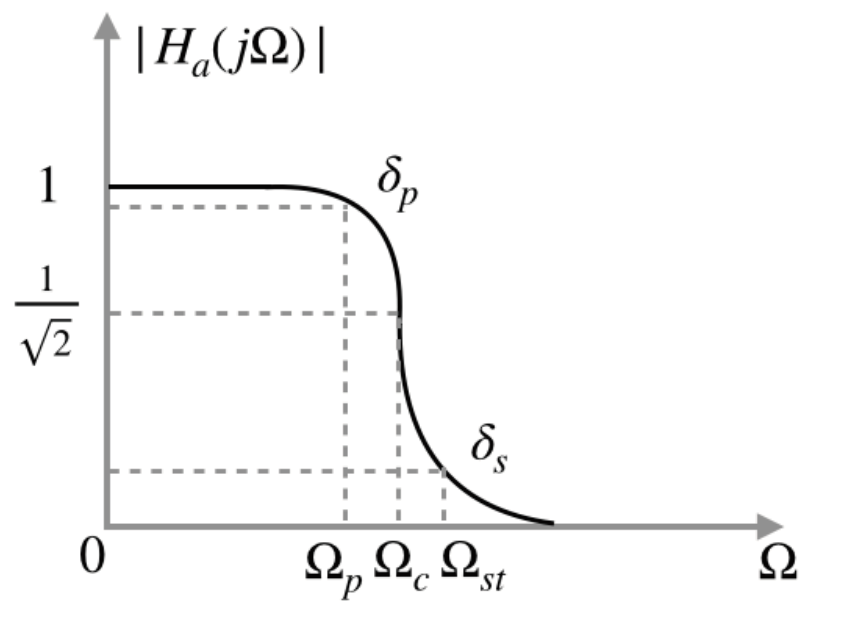
\includegraphics[width=0.33\textwidth]{filter_amp_square.png}
\caption{幅度平方函数和衰减和通带阻带频率关系}
\end{figure}
\section{Butterworth filter}
滤波器阶数$N$为
\begin{equation}
  N=\frac{\lg{\bigg(\frac{10^{0.1\cdot A_p}-1}{10^{0.1\cdot A_s}-1}\bigg)}}{2\cdot\lg{\frac{\Omega_p}{\Omega_s}}}
\end{equation}
截止频率$\Omega_c$
\begin{align}
  \Omega_c&=\frac{\Omega_p}{(10^{0.1\cdot A_p}-1)^{\frac{1}{2N}}}
  \\ &=\frac{\Omega_s}{(10^{0.1\cdot A_s}-1)^{\frac{1}{2N}}}
\end{align}
前者为通带指标, 后者为阻带指标. 

第$k$个极点公式, 有$N$(阶数)个极点
\begin{equation}
  s_k=\Omega_c\cdot e^{j\cdot\frac{\pi}{2}\cdot (1+\frac{2k-1}{N})}
\end{equation}
最后得到模拟滤波器的$H(s)$
\begin{equation}
  H(s)=\frac{\Omega_c^N}{\displaystyle\prod_{k=1}^{N}(s-s_k)}
\end{equation}
\section{模拟滤波器转数字滤波器}
\subsection{脉冲响应不变法}
冲激响应不变法 (Impulse-Invariant Method)

把模拟滤波器写成并联求和形式(或者说部分分式展开形式? )
\begin{align}
  H_a(s)=\displaystyle\sum_{k=1}^{N}\frac{A_k}{s-s_k}
\end{align}
此时可以进行Z变换为
\begin{equation}
  H(z)=\displaystyle\sum_{k=1}^{N}\frac{A_k}{1-e^{s_k\cdot T}\cdot z^{-1}}
\end{equation}
其中$T$指的是采样周期$f_s=\frac{1}{T}$
\subsection{双线性变换法}
可能会用到
\begin{equation}
  \underset{\text{数字角频率}}{\omega}=\underset{\text{模拟角频率}}{\Omega}\cdot T_s
\end{equation}

根据数字指标$\omega_p$和$\omega_s$代入到
\begin{equation}
  \Omega=\tan{\frac{\omega}{2}}
\end{equation}
得到\textbf{虚构的}模拟指标$\Omega_p$和$\Omega_s$, 然后设计出符合虚构的模拟指标的滤波器$H_a(s)$
直接运用双线性变换
\begin{equation}
  H(z)=H_a(s)\mid_{s=\frac{1-z^{-1}}{1+z^{-1}}}
\end{equation}
% \section{直接设计数字滤波器}
\chapter{FIR}
\section{FIR分类}
\begin{itemize}
  \item $h(n)$为奇或偶对称
  \item $N$的长度为奇数或偶数
\end{itemize}
\begin{equation}
  a=\frac{N-1}{2}
\end{equation}
被称为群延时
\subsection{偶对称脉冲响应}
\begin{equation}
  h(n)=h(N-1-n)
\end{equation}
系统的相位为
\begin{equation}
  \theta (\omega)=-\frac{N-1}{2}\cdot \omega
\end{equation}
又被称作第一类
\subsection{奇对称脉冲响应}
\begin{equation}
  h(n)=-h(N-1-n)
\end{equation}
\begin{equation}
  \theta (\omega)=-\frac{N-1}{2}\cdot \omega-\frac{\pi}{2}
\end{equation}
又被称作第二类
% Table generated by Excel2LaTeX from sheet 'Sheet1'
\begin{table}[H]
  \centering
  \caption{幅度函数的对称性}
    \begin{tabular}{c|cccc}
    滤波器 & N     & $A(\omega)$  & 零点    & 滤波器 \\
    \multirow{2}[0]{*}{$h(N-1-N)$} &     奇数  &  $\omega=0$和$\pi$偶对称     &  无     &  都可\\
          &   偶数    &  $\omega=0$偶对称 $\omega=\pi$ 奇对称     &  $A(\omega)=0$     &  LP和BP\\
    \multirow{2}[0]{*}{$-h(N-1-N)$} &   奇数    &   $\omega=0$和$\pi$奇对称    &    $A(0)=A(\omega)=0$   & BP \\
          &  偶数     &   $\omega=0$奇对称 $\omega=\pi$ 偶对称    &   $A(0)=0$    & HP和BP \\
    \end{tabular}%
  \label{tab:addlabel}%
\end{table}%

\section{窗函数设计法}
理想低通滤波器, 矩形窗
\end{document}